%Created on: May 21, 2014       Edited by: Wesley Kyle
%Edited on: Sept 10, 2015       Edited by: Peter Gimby - adding companion guide
%Edited on: May 16, 2016	Edited by: P. Gimby - fixed page numbering error.
%Edited on: May 20, 2016        Edited by: P. Gimby - replaced preamble with input from external file - added tages for easy removal of prelab questions
%Edited on: Aug 23, 2016        Edited by: W.Kyle - Corrected typos and formating issues
%Edited on: Sep 5, 2017		   Edited by: P. Gimby	- Corrected table/label overlap

% Beginning code for all standard physics latex documents

%Created on: May 8, 2014    Edited by: Wesley Kyle
%Edited on:	May 12, 2016	Edited by: P. Gimby - cleaned up the code to remove unneeded packages
%Edited on:	May 13, 2016	Edited by: P. Gimby - collected a few more packages used in 325.
%Edited on:	May 16, 2016	Edited by: P. Gimby - fixed page numbering error.
%Edited on: May 20, 2016	Edited by: Alex Shook - Added packages for 497

\documentclass[justified]{tufte-book}
\usepackage{graphicx} % allow embedded images
\setkeys{Gin}{width=\linewidth,totalheight=\textheight,keepaspectratio}
\usepackage{amsmath}  % extended mathematics
\usepackage{bm}  % bold font in math mode
\usepackage{longtable} %lets long tables flow into multiple pages instead of running off the page or having to break tables up manually
\usepackage{booktabs} % book-quality tables
\usepackage{units}    % non-stacked fractions and better unit spacing
\usepackage{multicol} % multiple column layout facilities
\usepackage{tikz} %for drawing nice pictures
\usepackage{indentfirst} % makes first line of each new section be indented
\usepackage{enumitem} % extended options for the enumerate environment
\usepackage{soul} % gives more typestting options like spacing, underline, and strike-through
\usepackage{marvosym} %extra symbols package
\usepackage{multirow} % for special table controls
\usepackage[singlelinecheck=false]{caption} % allow captions w/o figure number
\captionsetup{compatibility=false} % corrects in issue with the caption package
\usepackage{float} % allows for contorl over position of figures and tables
\allowdisplaybreaks % allows equations to span two pages if needed
\usepackage{mathrsfs} % fancy math symbols
\usepackage{multirow} % for special table controls
\usetikzlibrary{arrows,shapes,snakes,calc,patterns,3d} % addon to tikz
\usetikzlibrary{circuits.ee.IEC} % addon to tikz
\usepackage{pgfplots} % package for making plots of functions
\usepackage{gensymb} % symbols i,e. degrees
\usetikzlibrary{decorations.pathmorphing} % to draw the springs
\tikzset{circuit declare symbol = ac source}
\tikzset{set ac source graphic = ac source IEC graphic}
\usepackage{changepage} % allows for full page environment
\usepackage{comment} % allows comment tags for large sections

% define new page style that puts page numbers in the middle
%\begin{comment}
\fancypagestyle{custom}{
\fancyhf{} % clear all header and footer fields
\fancyheadoffset{0pt}
\fancyfootoffset{0pt}
\fancyfoot[C]{\thepage}
\renewcommand{\headrulewidth}{0pt}
\renewcommand{\footrulewidth}{0pt}}
\pagestyle{custom}
%\end{comment}

%below creates a new circuit symbol for AC sources
\tikzset{
         ac source IEC graphic/.style=
          {
           transform shape,
           circuit symbol lines,
           circuit symbol size = width 3 height 3,
           shape=generic circle IEC,
           /pgf/generic circle IEC/before background=
            {
             \pgftransformresetnontranslations
             \pgfpathmoveto{\pgfpoint{-0.8\tikzcircuitssizeunit}{0\tikzcircuitssizeunit}}
             \pgfpathsine{\pgfpoint{0.4\tikzcircuitssizeunit}{0.4\tikzcircuitssizeunit}}
             \pgfpathcosine{\pgfpoint{0.4\tikzcircuitssizeunit}{-0.4\tikzcircuitssizeunit}}
             \pgfpathsine{\pgfpoint{0.4\tikzcircuitssizeunit}{-0.4\tikzcircuitssizeunit}}
             \pgfpathcosine{\pgfpoint{0.4\tikzcircuitssizeunit}{0.4\tikzcircuitssizeunit}}
             \pgfusepathqstroke
            }
          }
        }
% end of circuit symbol
%\begin{document}
%%%end individual beginning code/,$d


%  \begin{titlepage}
%    \vspace*{\fill}
%    \begin{center}
%      \huge{{\bf TITLE1}}\\[0.4cm]
%      \huge{TITLE2}\\[0.4cm]
%      \LARGE{Laboratory Manual}\\[0.4cm]
%      \large{SEASON YEAR}
%    \end{center}
%    \vspace*{\fill}
%  \end{titlepage}
%\maketitle

%\begin{spacing}{0.5}
%\tableofcontents
%\end{spacing}

%NEW PHYS 497 PACKAGES AND COMMANDS

%Subcaption package: Allows subfigures to be placed side by side, and labeled with individual captions (Added June 1, 2016)
\usepackage{subcaption}

%Array package: Allows for addiation specifications in arrays (Added May 6, 2016)
\usepackage{array}

%newcolumntype: Allows one to specify a fixed column width (Added May 6, 2016)
\newcolumntype{L}[1]{>{\raggedright\let\newline\\\arraybackslash\hspace{0pt}}m{#1}}
\newcolumntype{C}[1]{>{\centering\let\newline\\\arraybackslash\hspace{0pt}}m{#1}}
\newcolumntype{R}[1]{>{\raggedleft\let\newline\\\arraybackslash\hspace{0pt}}m{#1}}

%circuits.logic.US, circuits.logic.IEC: For drawing logic gates in Tikz (Added May 6, 2016) 
\usetikzlibrary{circuits.logic.US,circuits.logic.IEC}

\newcommand{\PGT}{ %PGT: positive going transition
\begin{tikzpicture}
\draw[-angle 60] (0,0) -- (0,5pt);
\draw (0,5pt) -- (0,6pt) -- (5pt,6pt);
\draw (-5pt,0) -- (0,0);
\end{tikzpicture}
}





%TEST
\usepackage{geometry}
\pagestyle{fancy}

%\usepackage[caption=false]{subfig}

%\makeatletter
%\renewenvironment{figure}[1][htbp]{%
%  \@tufte@orig@float{figure}[#1]%
%}{%
%  \@tufte@orig@endfloat
%}

%\renewenvironment{table}[1][htbp]{%
%  \@tufte@orig@float{table}[#1]%
%}{%
%  \@tufte@orig@endfloat
%}
%\makeatother

% use instead of subfigure
\makeatletter
\newenvironment{multifigure}[1][htbp]{%
  \@tufte@orig@float{figure}[#1]%
}{%
  \@tufte@orig@endfloat
}
\makeatother

\makeatletter
\newenvironment{mainfigure}[1][htbp]{%
\@tufte@orig@float{figure}[#1]
\begin{adjustwidth}{}{-153pt}}
{\end{adjustwidth}\@tufte@orig@endfloat}%
\makeatother

\makeatletter
\newenvironment{maintable}[1][htbp]{%
\@tufte@orig@float{table}[#1]
\begin{adjustwidth}{}{-153pt}}
{\end{adjustwidth}\@tufte@orig@endfloat}%
\makeatother

%%%% Labatorial Cross-over labs need this code. This should be temporary PG Dec 7, 2016

\newcounter{questioncounter}
\setcounter{questioncounter}{0}
\newcounter{checkpointcounter}
\setcounter{checkpointcounter}{0}
\newcounter{figurecounter}
\setcounter{figurecounter}{0}
%%%%%%%%%%%%%%%%%%%%%%%%%%%%%%%%%%%%%%%%%%%%%%%%%%%%%%%

\newcommand{\checkpoint}{
 \fbox{\begin{minipage}{0.2\textwidth}
 %\includegraphics[width=0.5\textwidth]{stop}
 \end{minipage}
 \begin{minipage}{1.0\textwidth}
 {\bf CHECKPOINT \addtocounter{checkpointcounter}{1} \arabic{checkpointcounter}: Before moving on to the next part, have your TA check the results you obtained so far.}
 \end{minipage}}}

%%% end labatorial cross-over code.

% New environment for placing figure captions under the figure
%\makeatletter
%\newenvironment{mainfigure}{\textwidth}[1][htbp]{%
%\@tufte@orig@float{figure}[#1]%
%}{%
%\@tufte@orig@endfloat
%}
%\makeatother


\begin{document}

%%%start document%%% DO NOT REMOVE THIS LINE
\chapter{Spectroscopy}

\section{Equipment}

% first column
\begin{minipage}[t]{0.6\textwidth}
\begin{itemize}[noitemsep]
\item Introductory student spectroscope
\item 600 lines/mm diffraction grating
\item Spectrum tube power supply
\item Hydrogen and Helium Geissler tubes 
\end{itemize}
\end{minipage}
%second column
\begin{minipage}[t]{0.4\textwidth}
\begin{itemize}[noitemsep]
\item Low pressure Sodium lamp
\item Cadmium Osram lamp
\item Laboratory jack
\end{itemize}
\end{minipage}

\begin{marginfigure}[+1in]
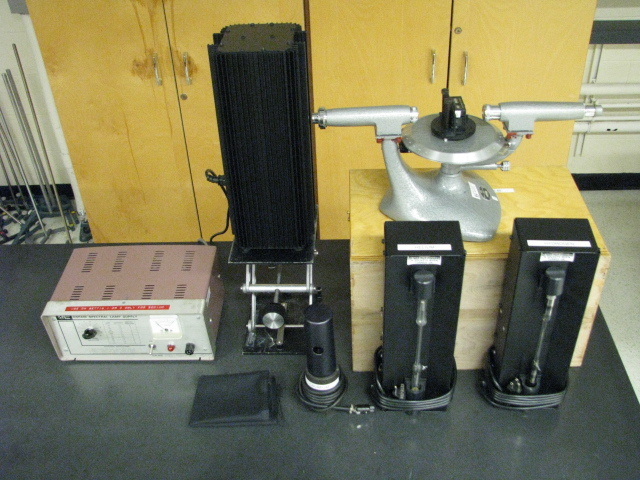
\includegraphics{Spectroscopy-Setup.jpg}
\caption{A photograph of the experimental setup.}
\label{fig:SPsetup}
\end{marginfigure}

\section{Preparation}
Review diffraction. Study the Bohr atom and the Bohr derivation of the Balmer formula. Understand the relationship between the energy difference of an electronic transition and the wavelength of the emitted photon.

\section{Goals of the Experiment}
\begin{itemize}
    \item To learn how to calibrate a spectroscope using a spectral source with known wavelengths.
    \item To use a spectroscope to measure wavelengths of spectral lines of unknown sources.
    \item 
\end{itemize}
%To learn how to calibrate a spectroscope using a spectral source with known wavelengths. To be able to measure wavelengths of spectral lines using a spectroscope.

\section{Theory}
An important issue in all experimental fields of physics is the nature of {\bf calibration}. How can one verify that a measurement device reports accurate values? How does one take readings from a measurement device and convert them to values of interest? For instance, in this experiment, how is the angle of diffraction that a spectroscope provides related and converted to wavelength, which is the desired parameter. In this experiment, the nature of calibration through spectroscopy is explored by setting up a spectroscope and then calibrating it with the spectral wavelengths of Hydrogen. The spectral wavelengths of Hydrogen are a reliable calibration source because these wavelengths are accurately calculated by the theory of quantum mechanics. Therefore, the calibration of the spectroscope is based on the assumption that quantum mechanics is correct. Afterwards, once the spectroscope is calibrated, the spectral lines of more complicated atoms like Helium, Sodium, and Cadmium are measured.

A description of the spectroscope and it's main component, a diffraction grating, are contained in sections I and II respectively. This is followed by a description of spectral lamps and their construction in section III. Lastly, the quantum mechanical description of the Hydrogen atom required for this experiment are contained in section IV, with a more complete version of the theory outlined in the appendix.

\section{I - The Spectroscope}
In 1666, Isaac Newton passed sunlight through a glass prism to observe, what he called, a "spectrum" of colours. It was this experiment that lead to what is now known as {\bf spectroscopy}. Spectroscopy is the study of the electromagnetic spectrum and the emission and absorption of electromagnetic radiation. The science of spectroscopy is useful in many areas that requires the analysis of light. Astronomers use spectroscopy to determine the composition of stars and galaxies. Much of what is known about the Sun comes from the analysis of its spectrum. One of the first to study the Solar spectrum was Joseph von Fraunhofer. In 1814 he found that the spectrum of the Sun contained fine, dark lines which, are now known to be caused by the absorption of light by gases in the Sun. A pattern of dark lines in a continuous spectrum is called an {\bf absorption} spectrum. The opposite, discrete coloured lines on a dark background, is called an {\bf emission} spectrum and is caused by the emission of light by excited atoms.

The spectral lines visible to the human eye vary from violet to red in colour. The most common method of observing spectra is through the use of a {\bf spectroscope}. This type of instrument enables the user to observe the spectrum of various elements and facilitates the measurement of the wavelengths of each spectral line. Figure \ref{fig:sp1} is a diagram of the Introductory Student Spectroscope used in this experiment. Light passes through the {\bf slit} and the {\bf collimator}. It is then bent by the {\bf diffraction grating}. The {\bf Telescope} is connected to a rotatable arm so that it can be moved to allow the bent light to pass through it. A vernier on the telescope is then used to measure the angle at which the incident light is diffracted. Then this angle can be used to find the wavelength of the selected emission line. Encircling the base of the grating table is a 360 degree scale used to make measurements in conjunction with the vernier scale, which is fixed to the telescope arm.

\begin{figure}[t]
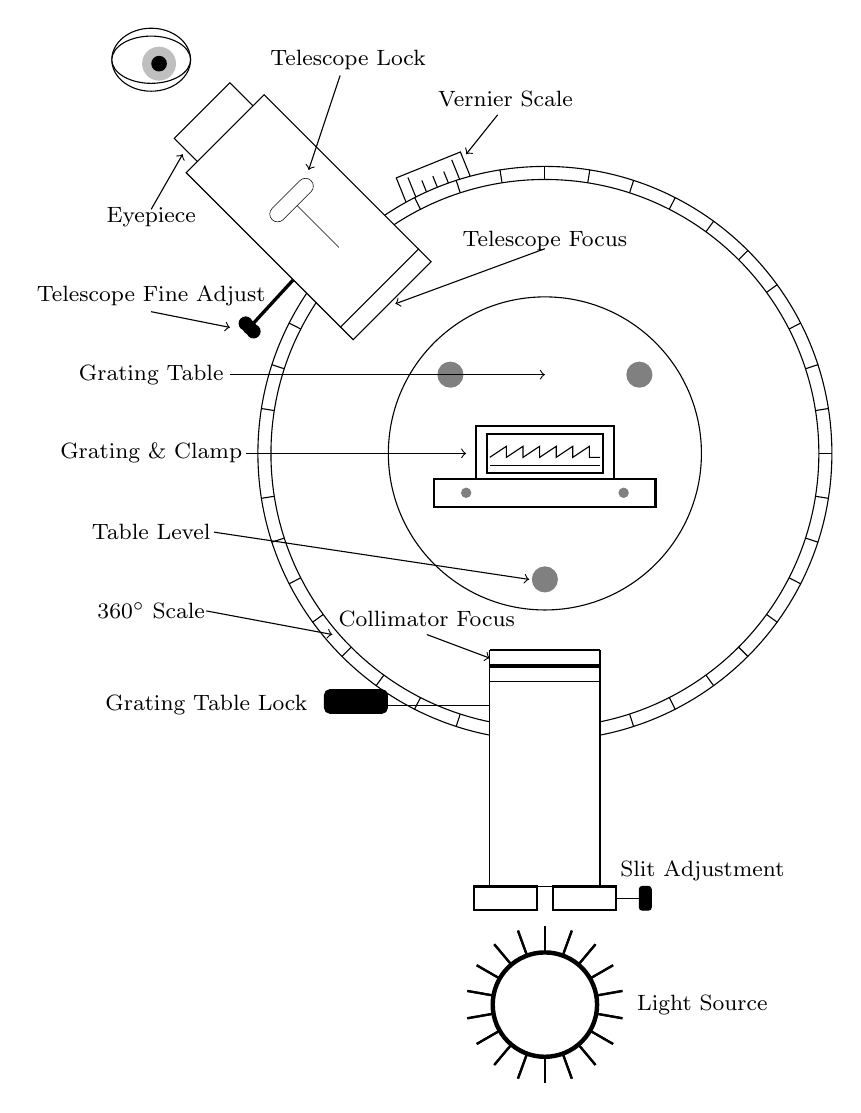
\begin{tikzpicture}
%vernier scale
\begin{scope}[rotate=22,shift={(0cm,3.6cm)}]
\node[rotate=22,shape=rectangle,minimum width=25,minimum height=20,draw]at(0,0){};
\draw(-.3,.3)--(-.3,-.2)--(.3,-.2)--(.3,.3);
\draw(-.15,-.2)--(-.15,.2);
\draw(0,-.2)--(0,.2);
\draw(.15,-.2)--(.15,.2);
\end{scope}

\node[shape=circle,draw=black,fill=white,scale=22]at(0,0){}; %outer ring
%some scale tics on the outer ring
\foreach \r in {0,...,19}
{
\draw[rotate=\r*9](0,-3.65)--(0,3.65);
}
\node[shape=circle,draw=black,fill=white,scale=21]at(0,0){}; %outer ring
\node[shape=circle,draw=black,fill=white,scale=12]at(0,0){}; %inner ring
%telescope
\node[shape=rectangle,fill=white,draw=black,minimum width=1cm,minimum height=1cm
,rotate=45]at(-4,4){};
\node[shape=rectangle,fill=white,draw=black,minimum width=1.4cm,minimum height=3cm
,rotate=45]at(-3,3){};
\draw[](-2.6,1.6)--(-1.6,2.6);
%collimator
\node[rectangle,fill=white,draw,minimum width=1.4cm,minimum height=3cm]at(0,-4){}; %tube
\draw[ultra thick](-.7,-2.7)--(.7,-2.7);
\draw[thick](-.7,-2.5)--(.7,-2.5);
\draw(-.7,-2.9)--(.7,-2.9);
\draw[thick](-.9,-5.8)rectangle(-.1,-5.5);
\draw[thick](.1,-5.8)rectangle(.9,-5.5);
%table levels
\node[circle,scale=1,fill=gray]at(0,-1.6){};
\node[circle,scale=1,fill=gray]at(-1.2,1){};
\node[circle,scale=1,fill=gray]at(1.2,1){};
%light source
\foreach \r in {0,...,17}
{
\draw[thick,shift={(0cm,-7cm)},rotate=\r*20](0,-1)--(0,1);
}
\node[circle,scale=4,draw,fill=white,ultra thick]at(0,-7){};
%grating
\node[rectangle,thick, minimum width=50,minimum height=20,draw]at(0,0){};
\node[rectangle,thick, minimum width=80,minimum height=10,draw,fill=white]at(0,-.5){};
\node[circle,fill=gray,scale=.4]at(-1,-.5){};
\node[circle,fill=gray,scale=.4]at(1,-.5){};
\node[rectangle,thick, minimum width=42,minimum height=14,draw]at(0,0){};
\draw[](-.7,-.15)--(.7,-.15);
\draw[decorate,decoration={saw,segment length=6, amplitude=4}](-.7,-.05)--(.7,-.05);
%adjustment knobs
%Telescope fine adjust
\draw[very thick](-3.2,2.2)--(-3.75,1.6);
\node[circle,fill,draw,scale=.5]at(-3.75,1.6){};
\node[circle,fill,draw,scale=.5]at(-3.8,1.65){};
\node[circle,fill,draw,scale=.5]at(-3.7,1.55){};
% Telescope lock knob
\begin{scope}[rotate=45,shift={(0cm,3.7cm)}]
\draw[very thin](0,0)--(0,.75);
\draw[very thin](-.25,.75)--(.25,.75);
\draw[very thin](-.25,.95)--(.25,.95);
\draw[very thin](.25,.75) arc (-90:90:.1);
\draw[very thin](-.25,.95) arc (90:270:.1);
\end{scope}
%Grating table lock knob
\draw[rounded corners=2,fill](-2.8,-3.3)rectangle(-2,-3);
\draw[very thin](-2,-3.2)--(-.7,-3.2);
%slit adjustment
\draw[](.9,-5.65)--(1.2,-5.65);
\draw[rounded corners=1,fill](1.2,-5.8)rectangle(1.35,-5.5);
%eyeball
\draw[](-5,5) ellipse(5mm and 4mm);
\draw[fill=white](-5,5) ellipse(5mm and 3mm);
\node[circle,scale=1.3,fill=lightgray]at(-4.9,4.95){};
\node[circle,scale=.6,fill]at(-4.9,4.95){};
%labels
\node[font=\footnotesize]at(-5,3){Eyepiece};
\draw[->,thin](-5,3.1)--(-4.6,3.8);
\node[font=\footnotesize]at(-5,2){Telescope Fine Adjust};
\draw[->,thin](-5,1.8)--(-4,1.6);
\node[font=\footnotesize]at(-5,1){Grating Table};
\draw[->,thin](-4,1)--(0,1);
\node[font=\footnotesize]at(-5,0){Grating \& Clamp};
\draw[->,thin](-3.8,0)--(-1,0);
\node[font=\footnotesize]at(-5,-1){Table Level};
\draw[->,thin](-4.2,-1)--(-.2,-1.6);
\node[font=\footnotesize]at(-5,-2){360$^{\circ}$ Scale};
\draw[->,thin](-4.3,-2)--(-2.7,-2.3);
\node[font=\footnotesize]at(-4.3,-3.2){Grating Table Lock};
\node[font=\footnotesize]at(-2.5,5){Telescope Lock};
\draw[->,thin](-2.6,4.8)--(-3,3.6);
\node[font=\footnotesize]at(-.5,4.5){Vernier Scale};
\draw[->,thin](-.6,4.3)--(-1,3.8);
\node[font=\footnotesize]at(0,2.7){Telescope Focus};
\draw[->,thin](0,2.6)--(-1.9,1.9);
\node[font=\footnotesize]at(-1.5,-2.1){Collimator Focus};
\draw[->,thin](-1.5,-2.3)--(-.7,-2.6);
\node[font=\footnotesize]at(2,-5.3){Slit Adjustment};
\node[font=\footnotesize]at(2,-7){Light Source};
\end{tikzpicture}
\caption{A diagram of the spectrometer used in this experiment.}
\label{fig:sp1}
\end{figure}

Before the spectroscope can be used to measure the angles of spectral lines it must be adjusted to ensure that accurate results are obtained. To begin, the telescope is focused on a distant object, using the {\bf Telescope focus}. The telescope is then lined up with the slit in the end of the collimator, and the {\bf Collimator focus} is adjusted until the slit comes into sharp focus. In this way only parallel rays of light pass through the {\bf diffraction grating}.

\section{II - Diffraction Gratings}
A diffraction grating is sometimes known as a "super prism". When mixed light passes through a prism the individual wavelengths of light are bent at different angles. A prime example of a prism is raindrops. When sunlight passes through drops of rain it is diffracted, resulting in a rainbow which shows the different colours that make up sunlight. A diffraction grating  can be imagined as a flat surface with thousands of grooves which each act as prism. As seen in Figure \ref{fig:sp2}, the diffraction grating used in this experiment has a sawtooth pattern instead of simple grooves. It can be shown that this pattern, called a {\bf blazed grating}, spreads light away from the centre more effectively than grooves.

When light from an emission spectrum passes through a blazed diffraction grating the light is split into its constituent colours. Atomic spectra are observed as a series of lines because of the constructive interference of the light waves once they have passed through the diffraction grating. Destructive interference produces what is observed between spectral lines, that is, nothing. Constructive interference occurs when two or more waves of light, of equal wavelength, are superimposed in phase, resulting in a maxima, or a spectral line. In order for two identical light waves, diffracted by side by side grooves, to be in phase they must travel a distance that differs by one wavelength after they have been diffracted. As seen in Figure \ref{fig:sp2}, this implies that the distance, p, must be an integer multiple of the wavelength. Therefore for constructive interference the requirement is that

\begin{equation}
dsin\theta=m\lambda\hspace{10mm}m=0,\pm1,\pm2,...
\label{equ:sp1}
\end{equation}

\begin{marginfigure}
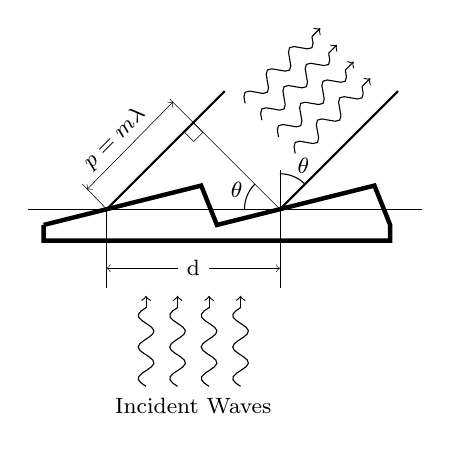
\begin{tikzpicture}
\draw[very thin](0,0)--(5,0);
\draw[ultra thick](.2,-.2)--(2.2,.3)--(2.4,-.2)--(4.4,.3)--(4.6,-.2)
--(4.6,-.4)--(.2,-.4)--(.2,-.2); %grating
\draw[thick](1,0)--(2.5,1.5);
\draw[thick](3.2,0)--(4.7,1.5);
\node[rectangle,draw,rotate=45,scale=.7,very thin]at(2.105,.975){}; %right angle
%demarcation lines
\draw[very thin](1.8,1.4)--(3.2,0);
\draw[very thin](1,0)--(1,-1);
\draw[very thin](3.2,.5)--(3.2,-1);
\draw[very thin](1,0)--(.69,.32);
\draw[<->,very thin](.75,.25)--(1.84,1.36);
\draw[<->,very thin](1,-.75)--(3.2,-.75);
\draw(2.75,0) arc (-180:-225:.45);
\draw(3.2,.45) arc (90:45:.45);
%labels
\node[font=\footnotesize,rotate=45]at(1.1,.9){$p=m\lambda$};
\node[font=\footnotesize,fill=white]at(2.1,-.75){d};
\node[font=\footnotesize]at(2.65,.25){$\theta$};
\node[font=\footnotesize]at(3.5,.55){$\theta$};
\node[font=\footnotesize]at(2.1,-2.5){Incident Waves};
%waves
\foreach \r in {0,1,2,3}
{
\draw[domain=0:1.,rotate=90,shift={(-2.25cm,-1.5cm-\r*.4 cm)}]
plot(\x,{.1*sin(\x*900)});
\draw[->](1.5+\r*.4,-1.25)--(1.5+\r*.4,-1.1);
}
\begin{scope}
\foreach \y in {0,1,2,3}
{
\draw[domain=0:1.2,rotate=45,shift={(2.9cm,-1cm-\y*.3 cm)}]
plot(\x,{.1*sin(\x*900)});
\draw[rotate=-45,->,shift={(-.5cm,5.35cm)}](1.5+\y*.3,-1.25)--(1.5+\y*.3,-1.1);
}
\end{scope}
\end{tikzpicture}
\caption{Diffraction of incident light by grating.}
\label{fig:sp2}
\end{marginfigure}

\noindent where d is the {\bf line spacing}, that is, the distance from one point on a groove to the same point on the neighboring groove. Note that the number given on the top of the diffraction grating (600 lines/mm) is the {\bf line density} not the line spacing. Line density is the inverse of line spacing. The {\bf angle of deviation}, $\theta$, is the angle between the central maximum and the spectral line. The variable, m, indicates the {\bf order} of the spectral lines. First order spectral lines ($m=\pm1$) are those found closest to the central maximum. As the telescope arm moves away from the central maximum, a point is reached where the spectral lines begin to repeat. These are known as the second order spectral lines ($m=\pm2$). Although second order maxima are visible, only first order maxima are used in this experiment. The sign of the order is positive or negative depending whether the spectrum is to the right or left of the central maxima. Equation \ref{equ:sp1} can be used to calculate the wavelength of a particular spectral line from the angle of deviation. For example, assuming a line spacing of 1000 lines/mm and a first order angle of deviation of 30$^{\circ}$ a wavelength of 500 nm is calculated.

\section{III - Spectral Sources}
The light from the emission spectrum that passes through the diffraction grating is generated by lamps called {\bf spectral sources}. Three different types of spectral sources are used in this experiment, the Hydrogen and Helium Geissler tubes, the low pressure Sodium lamp, and the Osram Cadmium lamp. In general, the glass parts of spectral lamps should not be touched. Touch only the metal ends of the tube. After a lamp is turned on move it as little as possible so that its lifetime is not shortened. When finished with a light source allow the lamp to cool for at least five minutes before moving it. Once a tube is removed from the power supply store it away immediately before starting to use a different tube. Due to their special nature, spectral lamps are expensive, costing hundreds to thousands of dollars, so they must be treated with care.

In this experiment the spectral lines of Hydrogen, calculated from quantum mechanics, are used to calibrate the spectroscope before confirming the spectral wavelengths of Helium, Sodium, and Cadmium. The accepted wavelengths for the primary visible spectral lines of these elements are presented in Table \ref{tab:sp1}.

\begin{margintable}
\normalsize
\begin{tabular}{|l|l|}
\hline
\multicolumn{2}{|c|}{Helium}                                        \\ \hline
\multicolumn{1}{|c|}{Wavelength (nm)} & \multicolumn{1}{c|}{Colour} \\ \hline
667.8150                              & bright red                  \\ \hline
587.5620                              & bright yellow\;\;\;\;\;               \\ \hline
501.5678                              & bright green                \\ \hline
471.3146                              & bright blue                 \\ \hline
447.1479                              & bright purple               \\ \hline
\end{tabular}
\end{margintable}

\begin{margintable}
\normalsize
\begin{tabular}{|l|l|}
\hline
\multicolumn{2}{|c|}{Sodium}                                        \\ \hline
\multicolumn{1}{|c|}{Wavelength (nm)} & \multicolumn{1}{c|}{Colour} \\ \hline
616.0747                              & bright red                  \\ \hline
615.4225                              & bright red                  \\ \hline
589.5924                              & bright yellow\;\;\;\;\;        \\ \hline
588.9950                              & bright yellow               \\ \hline
568.8205                              & lime                        \\ \hline
568.2633                              & lime                        \\ \hline
\end{tabular}
\end{margintable}

\begin{margintable}
\normalsize
\begin{tabular}{|l|l|}
\hline
\multicolumn{2}{|c|}{Cadmium}                                       \\ \hline
\multicolumn{1}{|c|}{Wavelength (nm)} & \multicolumn{1}{c|}{Colour} \\ \hline
643.8470                              & bright red                  \\ \hline
508.5822                              & bright green                \\ \hline
479.9912                              & bright light blue           \\ \hline
467.8149                              & bright blue                 \\ \hline
\end{tabular}
\caption{Spectral line wavelengths and apparent colours for Helium, Sodium, and Cadmium.}
\label{tab:sp1}
\end{margintable}

Helium Giessler tubes are constructed by filling a glass tube with a pure sample of the desired gas and then adjusting the pressure of the gas to yield maximum brightness. The glass tube is fitted with two electrodes, one at each end. The completed tube is clamped into a high voltage power supply. The high voltage creates an electric field between the electrodes which causes the valence electrons in the atoms to become excited. When the excited electrons lose energy they give off a mixed light containing all wavelengths that are characteristic of the element contained in the tube. Geissler spectral lamps should be turned off when not being used to lengthen their life. Be careful when handling a high voltage supply, do not touch any exposed metal parts. 

The construction of the Low Pressure Sodium tube is more complicated than the Geissler tube. Since Sodium is a solid at room temperature there is insufficient Sodium vapour present for the lamp to be started at any reasonable voltage (less that several thousand volts). It was found that by adding a noble gas mixture of 1.5\% Argon and 98.5\% Neon to the lamp, the starting voltage could be lowered to about 600 Volts. When a cold lamp is turned on a voltage "kick" is supplied to the discharge tube which generates enough charge carriers that the Argon and Neon become conductive. Once conduction begins, the voltage decreases and the discharges remain confined to the noble gases. As the noble gases discharge, heat is generated which eventually causes the Sodium to vaporize. The vaporized Sodium atoms are excited by the electric field present in the lamp. The noble gases are not excited any more because the valence electron of the Sodium is much easier to excite that any of the electrons in the noble gases. When using the Sodium lamp it is important to allow the lamp to warm up for at least ten minutes before making any measurements in order to ensure that the spectrum being measured is actually that of Sodium and not of Neon or Argon. The  Sodium lamp should be left on until all measurements are completed. Turning the lamp on and off will reduce its lifetime, and it is also time consuming as the lamp must be warmed up each time it is turned on.

The Osram Cadmium lamp functions in much the same way as the Low Pressure Sodium Lamp. The main differences are in the noble gas mixture used to start the lamp and the presence of Cadmium instead of Sodium. Do not touch the current setting on the Ealing Power supply. A current of one Ampere is sufficient to obtain a clear spectrum. As with the Low Pressure Sodium lamp, allow the lamp to warm up for at least ten minutes, and leave the lamp on until all measurements have been made.

\section{IV - The Hydrogen Atom}
One of the most commonly studied emission spectra is that of Hydrogen. With the simplest spectrum, Hydrogen is the most basic case of emission and absorption to study. Excited atoms can emit electromagnetic radiation at many wavelengths but for the purposes of this experiment, only the visible region of the electromagnetic spectrum is examined. The visible emission spectrum of Hydrogen is known as the {\bf Balmer Series}, named after a Swiss mathematician who first discovered their pattern.

Johann Balmer (1825-1898) was a secondary school mathematics teacher. For many years, scientists sought after a formula to predict the position of the emission lines of hydrogen. As an adept mathematician, Balmer was able to produce a formula that predicts the wavelength of Hydrogen spectral lines with great accuracy. His {\bf Balmer formula} takes the form

\begin{equation}
\dfrac{1}{\lambda}=R\left[\dfrac{1}{2^2}-\dfrac{1}{n^2}\right],\hspace{4mm}n=3,4,5,...
\label{equ:sp2}
\end{equation}

\noindent where R is now called {\bf Rydberg's constant} and each integer, n, corresponds to an observed Hydrogen spectrum line. At the time, no one was able to provide an explanation for this formula. A proper explanation was not available until the Danish physicist, Niels Bohr (1885-1962) provided his theory of the atom (see the appendix for details) which demonstrated that

\begin{equation}
R=\dfrac{m_ee^4Z^2}{8\varepsilon^2_0h^3c}
\label{equ:sp3}
\end{equation}

\noindent where Z is the atomic number of the atom. With these equations it is possible to calculate the wavelengths of the visible spectrum lines of the Hydrogen atom.

\section{Experimental Procedure}
\begin{enumerate}

\item Remove the diffraction grating and its holder from the spectroscope. It is extremely important not to touch {\bf any} of the lenses or the diffraction grating. If cleaning of any lens on either the telescope or the collimator is required see the laboratory instructor. {\bf Do not use fingers or articles of clothing to clean the optical equipment as this will only result in scratching the optics}. The diffraction grating {\bf cannot} be cleaned at all, so handle it only by its frame.

\item The telescope must be focused for parallel light rays and the crosshairs must be put into focus. First slide the eyepiece on the telescope in or out and bring the crosshairs into sharp focus. Next, focus the telescope on a distant object across the room or out a window.

\item Use the Hydrogen lamp as the calibration light source and place it so that the light from it passes through the slit in the collimator. Aim the telescope at the slit and gently move the lamp until the slit is at its brightest. Adjust the collimator focus until the slit is in sharp focus. In this way the spectrum being measured uses only light parallel to the slit. Align the cross-hairs in the eyepiece with the slit. Do not change the focus of the telescope or the collimator, or rotate the eyepiece for the remainder of the experiment, as this affects the apparent position of the centre slit. Do not move the telescope by touching the eyepiece or the chrome part of the telescope, as this could change the focus of telescope.  

\item Replace the diffraction grating into its holder. The bolts for the diffraction grating holder should be facing the collimator, and the diffraction grating frame should be placed in the holder so that the diffraction grating is as close to the holder as possible. The idea here is that the diffraction grating needs to pass through the centre of the grating table as seen in Figure \ref{fig:sp1}. 

\begin{marginfigure}
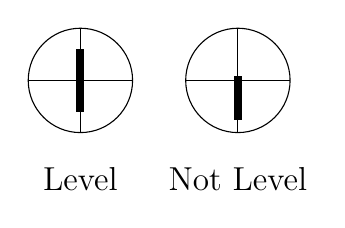
\begin{tikzpicture}
\node[draw,circle,scale=4]at(-1,0){}; %circle 1
\node[draw,circle,scale=4]at(1,0){}; %circle 2
%crosshairs
\draw(-1,-.66)--(-1,.66);
\draw(1,-.66)--(1,.66);
\draw(-1.66,0)--(-.33,0);
\draw(.33,0)--(1.66,0);
%spectral line
\draw[line width=1mm](-1,-.4)--(-1,.4);
\draw[line width=1mm](1,-.5)--(1,.05);
%labels
\node[font=\large]at(-1,-1.25){Level};
\node[font=\large]at(1,-1.25){Not Level};
\end{tikzpicture}
\caption{Levelling the grating table.}
\label{fig:sp3}
\end{marginfigure}

\item Turn the telescope and look at spectral lines that are far away from the center angle (choose second order lines if possible). Using the three grating table leveling screws on the bottom of the grating table, adjust the level of the table until the lines are vertically in the middle of the telescope as shown in Figure \ref{fig:sp3}. Move the  telescope to the other side of centre and adjust the lines until they are also centered. This adjustment may have be repeated several times on each side.

\item Look through the telescope and adjust the width of the slit. Take note of which side of the slit moves. All measurements should be taken from the side of the light line that {\bf does not} move. By doing this the width of the slit can be changed during the experiment. The slit width adjustment is used to adjust the amount of light that is allowed to pass into the collimator, as different amounts of light are useful in different situations. Some lines are close together and will overlap if the slit is too wide, in which case a narrow slit is required in order to resolve all of the lines that are present. On the other hand some lines are very dim. In such a case a wide slit is better in order for the spectral line to be bright enough that it can be seen.

\item Align the diffraction grating so it is perpendicular to the collimator as seen in Figure \ref{fig:sp2}. This is done by rotating the grating table. If the diffraction grating is not perpendicular, the angle of deviation of the spectral lines will differ between the two sides of the centre maximum. Choose any line in the spectrum and rotate the grating until the angle of deviation is the same on the left spectrum as the right spectrum. This step may need to be repeated several times in order to obtain satisfactory results.   

\item Measure the angle of the centre maximum. Align the cross-hairs with the stationary edge of the slit. Use the vernier to measure the angle of the maximum. A magnifying glass has been provided to assist in reading the vernier. All angles of diffraction are measured with respect to this centre angle. Each angle of diffraction is subtracted from the centre angle and the absolute value of that angle is the angle of deviation. The angle of deviation is then used to determine wavelengths of spectral lines using Equation \ref{equ:sp1}.
 
\item Use the Hydrogen spectral lamp to check the performance of the diffraction grating. The measured angle of deviation, along with Equation \ref{equ:sp1}, can be used to calibrate the spectroscope. If Equation \ref{equ:sp1} holds, a plot of $\lambda$ versus $sin(\theta)$ should yield a straight line with slope d and an intercept of zero. Using wavelengths calculated in the prelab and measured angles of deviation, make a quick plot of $\lambda$ versus $sin(\theta$) (errors need not be included here). Check that the slope of this line corresponds to approximately 600 lines/mm.

\item The spectroscope is now adjusted, checked, and ready for analyzing other spectra. Turn on one of the Helium, Sodium, or Cadmium lamps and shine the light through the slit in the collimator. Measure the angle of deviation, on one side of the center maximum, for the lines listed in Table \ref{tab:sp1}.

\item Repeat these measurements for the other two spectral lamps.

\end{enumerate}

\section{Error Analysis}
Usually $u(\theta)$ would be half the smallest division of the vernier on spectroscope, however there are other factors that add to the error. First, it is hard to take measurements from the same part of the spectral line each time a measurement is made. Second, as the eye moves back and forth across the eyepiece the cross-hairs move, therefore in order to get precise measurements the eye would have to be in exactly the same place for each measurement. Third, some lines are not very intense making them hard to see, and lining the cross-hairs up becomes difficult. Fourth, the crosshairs have a thickness which introduces an uncertainty in any visual measurement. Fifth, the condition of the grating, i.e., smudges, scratches, etc., can introduce visual abberrations like smearing. Finally, the spectroscope and diffraction grating used cannot distinguish between spectral lines that are too close together. This is a limitation of the diffraction grating construction as well as the magnification of the telescope. For example, the lines of the Sodium doublet differ by about half a nanometer and they are very close to appearing as one line. For these reasons, take the error in measurements of angles for this spectroscope to be 0.2$^{\circ}$. The uncertainty in the line density of 600 lines/mm for the diffraction grating as given by the manufacturer is unknown, however an error of about 5 lines/mm has been found to be reasonable. Either the manufacturer's line density error of 5 lines/mm, or the line density and error determined by the grating performance check can be used. Note, that {\bf $u(\theta)$ must be in radians} when calculations are being made. All other errors should be propagated using an appropriate method. 

\section{To be handed in to your laboratory instructor.}

%%% begin prelab %%%
\section{Prelab}

\begin{enumerate}

\item With Equation \ref{equ:sp3}, compute the numerical value of the Rydberg constant of Hydrogen with units.

\item Using Equation \ref{equ:sp2}, compute the visible spectral wavelengths of the Hydrogen spectrum and look up which color these wavelengths correspond to.

\item If the angle of deviation for a first order spectral line is 20 degrees 17 minutes, what is the wavelength of the corresponding spectral line, assuming the diffraction grating is 600 lines/mm.

\item \item Use uncertainty analysis to determine what uncertainty would be expected for measurements of wavelength with the spectroscope? (In other words, estimate what is the smallest wavelength separation that can be resolved.) Assume that the diffraction grating has 600 lines/mm and you are looking at wavelengths from the range between 400~nm and~700 nm. Use the uncertainty estimates outlined in the error analysis section. Will you be able to reliably resolve all the spectral lines of helium, sodium, and cadmium?  If not, list what sources of uncertainty would need to be decreased.

\end{enumerate}
%%% end prelab %%%

\section{{\bf Data Requirements}}
\begin{enumerate}[resume]

\item Notes and observations from the setup and alignment of the spectroscope (steps 1-7). 

\item A table of data for the Hydrogen lamp as a performance check of the diffraction grating, including calibration source, center angle, colour, angle of diffraction, angle of deviation, and theoretical wavelength together with errors (procedure step 9).


\section{Calculations and Analysis}

\item A graph of $\lambda$ (theoretical wavelength) versus $sin(\theta)$ and a value, with error, for the line spacing, $d$, of the diffraction grating (procedure step 9).

\item Tables of data from the Helium, Sodium, and Cadmium lamps, including center angle, colour, angle of diffraction, angle of deviation, and measured wavelength, together with errors (procedure steps 10 and 11).

\section{Discussion}

\item A comparison of the measured diffraction grating spacing with the expected value.

\item A discussion of the performance of the diffraction grating and which method of wavelength determination is preferred; using the manufacturers specified grating spacing or the measured grating spacing instead? Which error is preferred; the one in the error analysis section or the measured value?

\item A comparison of the spectral wavelengths measured for Helium, Sodium, and Cadmium, with the accepted values.

\end{enumerate}

\section{Appendix}

One of the most commonly studied emission spectra is that of Hydrogen. With the simplest spectrum, Hydrogen is the most basic case of emission and absorption to study. Excited atoms can emit electromagnetic radiation at many wavelengths but for the purposes of this experiment, only the visible region of the electromagnetic spectrum is examined. The visible emission spectrum of Hydrogen is known as the {\bf Balmer Series}, named after a Swiss mathematician who first discovered their pattern.

Johann Balmer (1825-1898) was a secondary school mathematics teacher. For many years, scientists sought after a formula to predict the position of the emission lines of hydrogen. As an adept mathematician, Balmer was able to produce a formula that predicts the wavelength of Hydrogen spectral lines with great accuracy. His {\bf Balmer formula} takes the form

\begin{equation}
\dfrac{1}{\lambda}=R\left[\dfrac{1}{2^2}-\dfrac{1}{n^2}\right],\hspace{4mm}n=3,4,5,...
\label{equ:sp4}
\end{equation}

\noindent where R is now called {\bf Rydberg's constant} and each integer, n, corresponds to an observed Hydrogen spectrum line. At the time, no one was able to provide an explanation for this formula. A proper explanation was not available until the Danish physicist, Niels Bohr (1885-1962) provided his theory of the atom.

In 1913 Niels Bohr proposed a theory for atomic structure that was able to account for the observed behaviour of atoms, including Balmer's formula. This theory contained several radical assumptions that violated concepts of classical physics. However, these new assumptions quickly came to be accepted because the theory agreed so well with experimental observations. Bohr assumed that an atom consisted of a massive positively charged nucleus and light negatively charged electrons.

So to explain atomic behaviour, the problem that Bohr addressed was the motion of a single electron about a nucleus of charge Z, where Z is the {\bf atomic number}, the number of protons in the nucleus. Following Bohr, assume that the electron moves in an orbit about the nucleus under the influence of the electrical attraction between the nucleus and the electron. Classically, such an orbiting electron is accelerating and so should radiate away electromagnetic energy continuously. Assume instead, that when an electron remains in a {\bf stable orbit} it does not radiate. Furthermore, assume that the nucleus is so much more massive than the electron, that the electron moves in a perfect circle about the exact center of the nucleus. Under these conditions, the electron follows the rules of classical physics. So the Coulomb attraction is the source of the centripetal acceleration of the orbiting electron, which gives the expression

\begin{equation}
\dfrac{1}{4\pi\varepsilon_0}\dfrac{e^2Z}{r^2}={m_ev^2}{r}
\label{equ:sp5}
\end{equation}

\noindent where $\varepsilon_0 = 8.85418782\times10^{-12}$ C$^2$ N$^{-1}$ m$^{-2}$ is the permittivity constant, $e = 1.60217646\times10^{-19}$ C is the electronic charge, r is the radius of the orbit, $m_e = 9.10938188\times10^{-31}$ kg is the mass of the electron, and $v$ is the velocity of the electron.

Moreover, not just any electron orbit is stable. Instead, assume that only certain values of electron orbital angular momentum give rise to stable orbits. The momentum condition for stable electron orbits is given by the expression

\begin{equation}
2\pi m_evr=nh,\hspace{4mm}n=1,2,3,...
\label{equ:sp6}
\end{equation}

\noindent where $h = 6.6260693\times10^{-34}$ m$^2$ kg s$^{-1}$ is Planck's constant. Equation \ref{equ:sp6} implies that electron orbits are quantized. Only certain orbits designated by the natural number n, now called the principal quantum number, are stable.

For each stable orbit, the electron has a fixed amount of energy. The kinetic energy, K, of the electron is found using Equation \ref{equ:sp5} to be

\begin{equation}
K=\dfrac{1}{2}m_ev^2=\dfrac{1}{8\pi\varepsilon_0}\dfrac{e^2Z}{r}
\label{equ:sp7}
\end{equation}

\noindent The potential energy, P, of the electron is the amount of work required to completely remove the electron from the nucleus. The work done to move the electron from its orbit to infinity is

\begin{equation}
P=-\int\limits_r^\infty\dfrac{1}{4\pi\varepsilon_0}\dfrac{e^2Z}{r^2}dr=-\dfrac{1}{4\pi\varepsilon_0}\dfrac{e^2Z}{r}
\label{equ:sp8}
\end{equation}

\noindent Since work is needed to move the electron from a lower orbit to a higher orbit, the potential energy is negative. By conservation of energy, the total energy of the electron, E, must be

\begin{equation}
E=K+P=-\dfrac{1}{8\pi\varepsilon_0}\dfrac{e^2Z}{R}
\label{equ:sp9}
\end{equation}

Equations \ref{equ:sp5} and \ref{equ:sp6} can be used to eliminate r from Equation \ref{equ:sp9} to yield the result

\begin{equation}
E=-\dfrac{m_ee^4Z^2}{8\varepsilon_0^2h^2}\dfrac{1}{n^2}
\label{equ:sp10}
\end{equation}

So evidently each electron orbit must have a quantized amount of energy specified by the quantum number n. The lowest energy level occurs for $n=1$. Note that the energy function is negative, so as $n$ increases, the energy becomes less negative until it reaches a maximum of zero at $n=\infty$. 

Now suppose that the electron only emits radiation when it changes orbits, somehow moving from a higher stable orbit to a lower stable orbit. Equation \ref{equ:sp10} implies that there must be a change in energy, $\delta$E, for this transition. Assume that the electron emits a photon of energy $\delta$E when the electron changes level. It seems reasonable to propose that the energy of this emitted photon is given by the Planck formula which is

\begin{equation}
\delta E=hf=\dfrac{hc}{\lambda}
\label{equ:sp11}
\end{equation}

\noindent where $c = 2.99792458\times10^8$ m s$^{-1}$ is the speed of light, f is the {\bf frequency} of the photon, and $\lambda$ is the {\bf wavelength} of the photon. Notice that the frequency of the emitted photon has nothing to do with the frequency with which the electron circles the nucleus.

Let the quantum number of the initial orbit be n$_i$ and the quantum number of the final orbit be $n_f$. Then substituting the initial and final energies given by Equation \ref{equ:sp9} into Equation \ref{equ:sp11} gives the result

\begin{equation}
\dfrac{1}{\lambda}=\dfrac{m_ee^4Z^2}{8\varepsilon_0^2h^3c}\left(\dfrac{1}{n_f^2}-\dfrac{1}{n_i^2}\right)
\label{equ:sp12}
\end{equation}

\noindent A comparison of Equation \ref{equ:sp12} with Equation \ref{equ:sp4} suggests that the Rydberg constant must be

\begin{equation}
R=\dfrac{m_ee^4Z^2}{8\varepsilon_0^2h^3c}
\label{equ:sp13}
\end{equation}

These results provide an explanation for the spectral lines of the Balmer series. When an atom is excited, by means of heat or otherwise, the increase in energy is accounted for when the electron jumps to a higher energy level. Emission lines result when the electron jumps back down to a lower energy level and emits a photon. In the case of Hydrogen, where Z=1, apparently the visible Balmer lines arise when an electron jumps down to the $n_f=2$ orbit. A comparison of the experimentally derived Rydberg constant with the constant predicted by Equation \ref{equ:sp13} would be a strong test of Bohr's atomic theory.

Figure \ref{fig:sp4} depicts some of the electron transitions in the Hydrogen atom. The figure includes transitions in the ultraviolet ({\bf Lyman series}), the visible ({\bf Balmer series}), and the infrared regions ({\bf Paschen series}) of the spectrum. The energy of each level is indicated on the left side and the respective quantum numbers on the right, as determined by Equation \ref{equ:sp10}. At the bottom of Figure \ref{fig:sp4} is a spectrum describing the location of each of the above mentioned series. The energy difference between each level is the energy an electron must gain in order to jump up to a specific level. Once the electron has jumped up, if it drops back down, a photon is emitted with exactly the same amount of energy as was initially gained. As there are only a specific number of energy levels, the photons created have correspondingly specific wavelengths giving rise to lines in the spectrum. Note that as wavelength increases, each series is similar to the previous one but with smaller line spacing, as seen at the bottom of Figure \ref{fig:sp4}. The Lyman series, with higher energy transitions, is located on the left, with the shorter wavelengths. On the opposite end, the Paschen series has much longer wavelengths as it contains lower energy differences in the transitions.

Each series, however, has an upper bound, known as the {\bf series limit}. For example, the Balmer series would require $n_f$ to be 2 and the Balmer series limit occurs when $n_i=\infty$. Conversely, if an electron initially sitting at $n_i=2$ gains an amount of energy equal to the series limit, called the {\bf ionization energy}, the electron reaches the level $n_{\infty}$. At this point the electron is completely removed from the Hydrogen atom and this Hydrogen atom is said to be {\bf ionized}. A series limit for the Lyman and Paschen series can be obtained similarly, where $n_i=1$ and $n_i=3$ for the Lyman and Paschen series, respectively. 

\begin{figure}
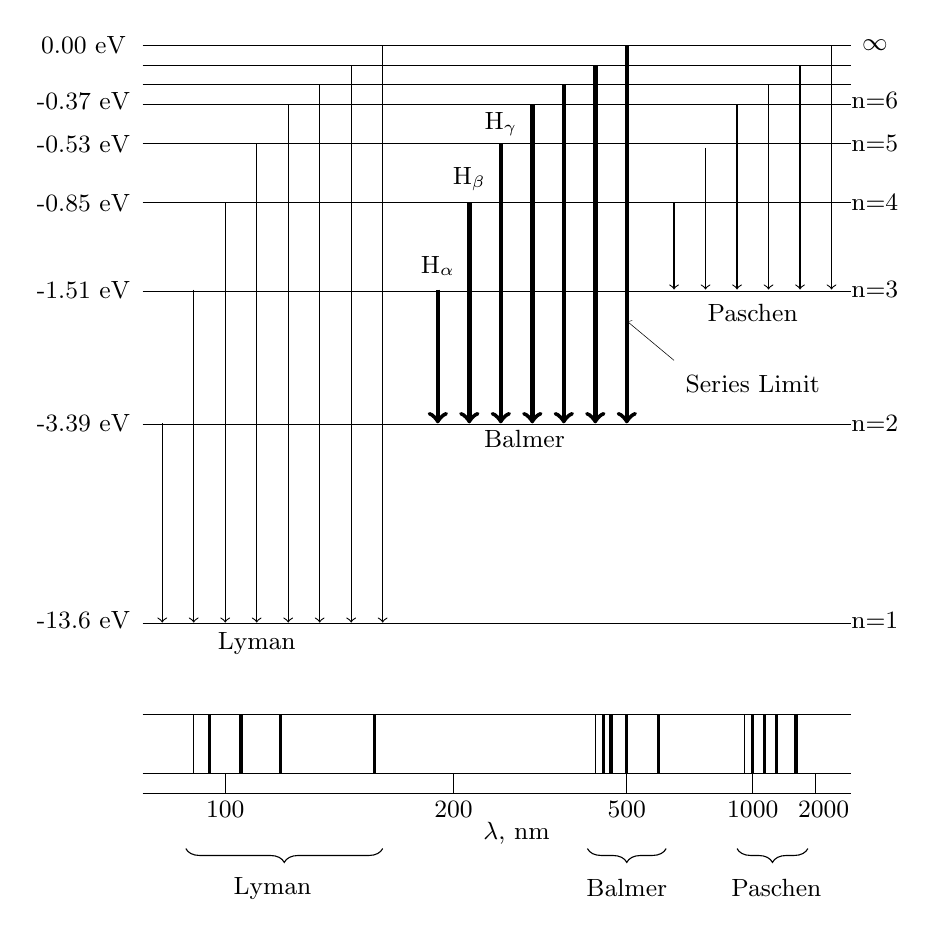
\begin{tikzpicture}
\draw[](0.25,0)--(9.25,0);
\draw[](0.25,-.25)--(9.25,-.25);
\draw[](0.25,-.5)--(9.25,-.5);
\foreach \x in {0,1,2,3,4,5}{
\draw[](0.25,.25-1.5^\x)--(9.25,.25-1.5^\x);
}
%lyman series
\draw[->](.5,-4.8)--(.5,-7.33);
\draw[->](.9,-3.1)--(.9,-7.33);
\draw[->](1.3,-2)--(1.3,-7.33);
\draw[->](1.7,-1.25)--(1.7,-7.33);
\draw[->](2.1,-.75)--(2.1,-7.33);
\draw[->](2.5,-.5)--(2.5,-7.33);
\draw[->](2.9,-.25)--(2.9,-7.33);
\draw[->](3.3,0)--(3.3,-7.33);
%balmer series
\draw[ultra thick,->](4,-3.1)--(4,-4.8);
\draw[ultra thick,->](4.4,-2)--(4.4,-4.8);
\draw[ultra thick,->](4.8,-1.25)--(4.8,-4.8);
\draw[ultra thick,->](5.2,-.75)--(5.2,-4.8);
\draw[ultra thick,->](5.6,-.5)--(5.6,-4.8);
\draw[ultra thick,->](6,-.25)--(6,-4.8);
\draw[ultra thick,->](6.4,0)--(6.4,-4.8);
%paschen series
\draw[->](7,-2)--(7,-3.1);
\draw[->](7.4,-1.3)--(7.4,-3.1);
\draw[->](7.8,-.75)--(7.8,-3.1);
\draw[->](8.2,-.5)--(8.2,-3.1);
\draw[->](8.6,-.25)--(8.6,-3.1);
\draw[->](9,0)--(9,-3.1);
%energies
\node[font=\small]at(-.5,0){0.00 eV};
\node[font=\small]at(-.5,-.7){-0.37 eV};
\node[font=\small]at(-.5,-1.25){-0.53 eV};
\node[font=\small]at(-.5,-2){-0.85 eV};
\node[font=\small]at(-.5,-3.1){-1.51 eV};
\node[font=\small]at(-.5,-4.8){-3.39 eV};
\node[font=\small]at(-.5,-7.3){-13.6 eV};
%principle quantum numbers
\node[font=\small]at(9.55,0){$\infty$};
\node[font=\small]at(9.55,-.7){n=6};
\node[font=\small]at(9.55,-1.25){n=5};
\node[font=\small]at(9.55,-2){n=4};
\node[font=\small]at(9.55,-3.1){n=3};
\node[font=\small]at(9.55,-4.8){n=2};
\node[font=\small]at(9.55,-7.3){n=1};
%labels
\node[font=\small]at(1.7,-7.6){Lyman};
\node[font=\small]at(5.1,-5){Balmer};
\node[font=\small]at(8,-3.4){Paschen};
\node[font=\small]at(8,-4.3){Series Limit};
\draw[very thin,->](7,-4)--(6.4,-3.5);
\node[font=\small]at(4,-2.8){H$_{\alpha}$};
\node[font=\small]at(4.4,-1.7){H$_{\beta}$};
\node[font=\small]at(4.8,-1){H$_{\gamma}$};
%spectrum
\draw[](.25,-8.5)--(9.25,-8.5);
\draw[](.25,-9.25)--(9.25,-9.25);
\draw[](.25,-9.5)--(9.25,-9.5);
%lyman spectral lines
\draw[](.9,-8.5)--(.9,-9.25);
\draw[very thick](1.1,-8.5)--(1.1,-9.25);
\draw[very thick](1.5,-8.5)--(1.5,-9.25);
\draw[very thick](2,-8.5)--(2,-9.25);
\draw[very thick](3.2,-8.5)--(3.2,-9.25);
%balmer spectral lines
\draw[](6,-8.5)--(6,-9.25);
\draw[very thick](6.1,-8.5)--(6.1,-9.25);
\draw[very thick](6.2,-8.5)--(6.2,-9.25);
\draw[very thick](6.4,-8.5)--(6.4,-9.25);
\draw[very thick](6.8,-8.5)--(6.8,-9.25);
%paschen spectral lines
\draw[](7.9,-8.5)--(7.9,-9.25);
\draw[very thick](8,-8.5)--(8,-9.25);
\draw[very thick](8.15,-8.5)--(8.15,-9.25);
\draw[very thick](8.3,-8.5)--(8.3,-9.25);
\draw[very thick](8.55,-8.5)--(8.55,-9.25);
%demarcation lines
\draw(1.3,-9.25)--(1.3,-9.5); %100
\draw(4.2,-9.25)--(4.2,-9.5); %200
\draw(6.4,-9.25)--(6.4,-9.5); %500
\draw(8,-9.25)--(8,-9.5); %1000
\draw(8.8,-9.25)--(8.8,-9.5); %2000
%labels
\node[font=\small]at(1.3,-9.7){100};
\node[font=\small]at(4.2,-9.7){200};
\node[font=\small]at(6.4,-9.7){500};
\node[font=\small]at(8,-9.7){1000};
\node[font=\small]at(8.9,-9.7){2000};
\node[font=\small]at(5,-10){$\lambda$, nm};
\node[font=\small]at(1.9,-10.7){Lyman};
\node[font=\small]at(6.4,-10.7){Balmer};
\node[font=\small]at(8.3,-10.7){Paschen};
\draw[decorate,decoration={brace,amplitude=5pt,mirror}](.8,-10.2)--(3.3,-10.2);
\draw[decorate,decoration={brace,amplitude=5pt,mirror}](5.9,-10.2)--(6.9,-10.2);
\draw[decorate,decoration={brace,amplitude=5pt,mirror}](7.8,-10.2)--(8.7,-10.2);
\end{tikzpicture}
\caption{Electronic de-excitation in Hydrogen with corresponding spectral lines.}
\label{fig:sp4}
\end{figure}

For example, an electron in the $n=3$ energy level dropping to the $n=2$ energy level emits a photon with $3.39-1.51=1.88$ eV. This transition is commonly known as the {\bf H-alpha line}. Planck's formula (Equation \ref{equ:sp11}) gives the wavelength and frequency of the emitted photon. The H-alpha line of the Balmer series is often used for the observation of the fine structure of active regions of the Sun.


\AtEndDocument{\clearpage\ifodd\value{page}\else\null\clearpage\fi} % forces even page count, for double siding

%%%end document%%% DO NOT REMOVE THIS LINE

%%%start companion guide%%% DO NOT REMOVE THIS LINE
\chapter{Spectroscopy - Companion Guide}

\section{Equipment}

% first column
\begin{minipage}[t]{0.6\textwidth}
\begin{itemize}[noitemsep]
\item Introductory student spectroscope
\item 600 lines/mm diffraction grating
\item Spectrum tube power supply
\item Hydrogen and Helium Geissler tubes 
\end{itemize}
\end{minipage}
%second column
\begin{minipage}[t]{0.4\textwidth}
\begin{itemize}[noitemsep]
\item Low pressure Sodium lamp
\item Cadmium Osram lamp
\item Laboratory jack
\end{itemize}
\end{minipage}

\section{Setup}
\begin{figure}
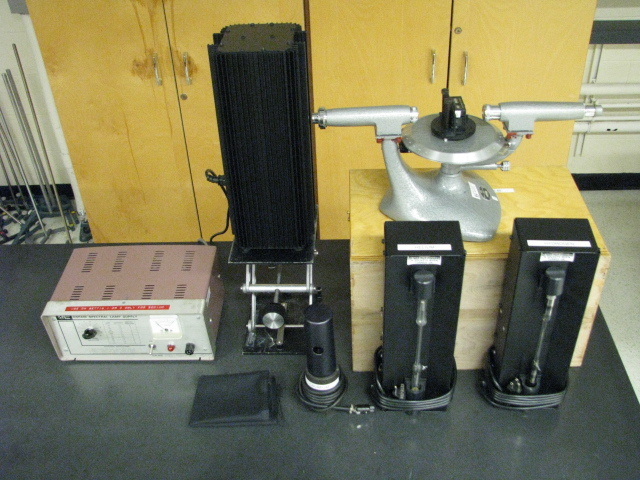
\includegraphics{Spectroscopy-Setup.jpg}
\caption{Equipment Setup}
\label{pic:SPsetup}
\end{figure}

Set up bench as shown in Figure \ref{pic:SPsetup}.

\section{Maintenance}

\begin{enumerate}
\item 
\item 
\end{enumerate}

\section{Critical Points of Failure}

There are currently no known critical points of failure.

\section{Notes to the Instructor}
\begin{enumerate}
\item It is very important for students' success that they calibrate the spectroscope carefully. Of primary importance is ensuring that the grating is perpendicular to the optical axis by checking that the angle of displacement to a reference line on one side is within 0.1$^{\circ}$ of the angle of displacement to the same line on the other side. If the difference is more than this, students will likely achieve unsatisfactory results.
\end{enumerate}

\section{Prelab Questions}
\begin{enumerate}

\item {\bf With Equation 3, compute the numerical value of the Rydberg constant of Hydrogen with units.}\newline

The value of the Rydberg constant for an atom of atomic number, Z, is given by

\small
\begin{align}
R&=\dfrac{m_ee^4Z^2}{8\epsilon_0^2h^3c}\\
&=\dfrac{(9.1\times10^{-31}kg)(1.6\times10^{-19}C)^4(1)^2}{8(8.9\times10^{-12}C^2N^{-1}m^{-2})^2(6.6\times10^{-34}m^2kgs^{-1})^3(3\times10^8ms^{-1})}\\
&=1.0917\times10^{7}m^{-1}
\label{equ:spcg1}
\end{align}
\normalsize

\item {\bf Using Equation 2, compute the visible spectral wavelengths of the Hydrogen spectrum and look up which color these wavelengths correspond to.}\newline

Using the following equation to calculate the wavelength of Balmer series transitions,

\begin{equation}
\dfrac{1}{\lambda}=R\left[\dfrac{1}{2^2}-\dfrac{1}{n^2}\right] \hspace{5mm}n=3,4,5,...
\label{equ:spcg2}
\end{equation}

\begin{table}[ht]
\center
\begin{tabular}{|l|l|l|}
\hline
\multicolumn{1}{|c|}{n} & \multicolumn{1}{c|}{Wavelength (nm)} & \multicolumn{1}{c|}{Colour} \\ \hline
3                       & 656.1                                & red                         \\ \hline
4                       & 486.0                                & indigo                      \\ \hline
5                       & 433.9                                & violet                      \\ \hline
6                       & 410.1                                & violet                      \\ \hline
7                       & 396.9                                & near UV                     \\ \hline
\end{tabular}
\caption{Results for prelab question 2.}
\label{tab:spcg1}
\end{table}

\noindent Students may include the 7-2 transition or not, depending on their definitions for the range of visible light.

\item {\bf If the angle of deviation for a first order spectral line is 20 degrees 17 minutes, what is the wavelength of the corresponding spectral line, assuming the diffraction grating is 600 lines/mm?}\newline

We manipulate the following equation,

\begin{equation}
dsin\theta=m\lambda\hspace{5mm}m=0,\pm1,\pm2,...
\label{equ:spcg3}
\end{equation}

\noindent and set the order, $m=1$, so that

\begin{equation}
\lambda=dsin\theta
\label{equ:spcg4}
\end{equation}

\noindent where $d=1/600$ and $\theta=20.28^{\circ}$. We get the result,

\begin{equation}
\lambda=577.7\hspace{1mm}nm
\label{equ:spcg5}
\end{equation}

\item {\bf Use error analysis to estimate what is the smallest wavelength separation that can be resolved. In otherwords, what uncertainty would be expected for measurements of wavelength with the spectroscope? Assume that the diffraction grating has 600 lines/mm and you are looking at wavelengths around 600nm. Use the error estimates outlined in the error analysis section. Will you be able to reliably resolve all the spectral lines of Helium, Sodium, and Cadmium? If not, list what sources of uncertainty would need to be decreased.}\newline

It is important when answering this question that the ideas of measurement uncertainty and resolution not be conflated, even though the phrasing of the questions appears to do so. The idea here is that a doublet may be able to be resolved in the student introductory spectrometer but the uncertainty in the measurement might preclude the ability to accurately measure the difference in angle between them. We then need to propagate the uncertainties listed in the Error Analysis section to find the uncertainty in any wavelength measurement. If two lines fall within this uncertainty, we can say that we would be unable to distinguish them {\it by measurement}. 

We begin by determining the linewidth, d, and the deviation angle, $\theta$, along with their corresponding uncertainties, u(d) and u($\theta$), respectively.

\begin{equation}
d=\dfrac{1}{600000\hspace{1mm}lines/m}=1.67\times10^{-6}
\label{equ:spcg6}
\end{equation}



\begin{align}
u(d)&=\dfrac{\partial d}{\partial n_{lines}}\cdot u(n_{lines})\\
&=\dfrac{1}{(600000\hspace{1mm}lines/m)^2}\cdot 5000\hspace{1mm}lines/m\\
&=1.39\times10^{-8}
\label{equ:spcg7}
\end{align}

\noindent So the line spacing, d, is expressed as $1.67\times10^{-6}\pm1.39\times10^{-8}$ m. Moving on to the angle, $\theta$, we are told that we are observing around wavelengths of 600 nm.

\begin{align}
\theta&=sin^{-1}(\dfrac{\lambda}{d})=sin^{-1}\left(\dfrac{600\times10^{-9}}{1.67\times10^{-6}}\right)\\
&=0.367\pm 0.0035\hspace{1mm}rad
\label{equ:spcg8}
\end{align}

\noindent We are told that the uncertainty in any angle measurement is $\pm 0.2^{\circ}$ which is $\pm 0.0035$ radians.

The expression we use for finding the uncertainty in the wavelength is derived from Equation \ref{equ:spcg3} with the order, m, taken to be $1$. We then apply the partial derivative formula for uncertainty and add the terms in quadrature.

\begin{align}
u(\lambda)&=\sqrt{\left(\dfrac{\partial \lambda}{\partial d}\cdot u(d)\right)^2+\left(\dfrac{\partial \lambda}{\partial \theta}\cdot u(\theta)\right)^2}\\
&=\sqrt{(sin(\theta)\cdot u(d))^2+(dcos(\theta)\cdot u(\theta))^2}\\
&=7.39\hspace{1mm}nm
\label{equ:spcg9}
\end{align}

So our uncertainty in any measurement of angle expresses itself as an uncertainty of $\pm5.65$ nm in the wavelength. This means that for the red, yellow, and lime Sodium doublets, the uncertainty of each measurement is larger than the separation between the lines.

\end{enumerate}


\section{Data Requirements}
\begin{enumerate}

\item {\bf Notes and observations from the setup and alignment of the spectroscope (steps 1-7).}\newline

Collimator and telescope were focused, crosshairs were brought into focus, grating table was balanced, and the grating was aligned to be perpendicular to the optical axis.

\item {\bf A table of data for the Hydrogen lamp as a performance check of the diffraction grating, including calibration source, center angle, colour, angle of diffraction, angle of deviation, and theoretical wavelength together with errors (procedure step 9).}\newline

\begin{maintable}[ht]
%\center
\begin{tabular}{|l|l|l|l|l|l|}
\hline
\multicolumn{1}{|c|}{Calibration Source} & \multicolumn{1}{c|}{$\theta_0$ (deg)} & \multicolumn{1}{c|}{Colour} & \multicolumn{1}{c|}{$\theta$ (deg)} & \multicolumn{1}{c|}{$\Delta\theta$ (deg)} & \multicolumn{1}{c|}{$\lambda$ (nm)} \\ \hline
Hydrogen                                 & 207.8                                 & violet                      & 222.2                               & 14.4$\pm$0.2                              & 414.5$\pm$6.61                      \\ \hline
                                         &                                       & violet                      & 223.0                               & 15.2$\pm$0.2                              & 437.0$\pm$6.69                      \\ \hline
                                         &                                       & indigo                      & 224.9                               & 17.1$\pm$0.2                              & 490.1$\pm$6.90                      \\ \hline
                                         &                                       & red                         & 231.2                               & 23.4$\pm$0.2                              & 661.9$\pm$7.68                      \\ \hline
\end{tabular}
\caption{Data collected for Hydrogen calibration.}
\label{tab:spcg2}
\end{maintable}

\item {\bf A rough graph of $\lambda$ (theoretical wavelength) versus sin($\theta$) and a value with error for the line spacing, d, of the diffraction grating (procedure step 9).}\newline

\begin{figure}
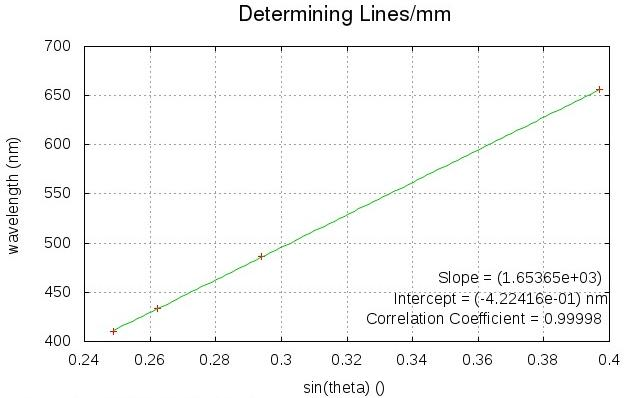
\includegraphics{Spectroscopy-calibration.jpg}
\caption{Rough linear plot of $\lambda$ vs. sin($\theta$). Here the slope is 1.65 $\mu$m which corresponds to 604.7 lines/mm, within the uncertainty of the manufacturers value of 600$\pm$5 lines/mm.}
\label{fig:spcg1}
\end{figure}

\item {\bf Tables of data from the Helium, Sodium, and Cadmium lamps, including center angle, colour, angle of diffraction, angle of deviation (procedure steps 10 and 11).}\newline

\begin{table}[ht]
\center
\begin{tabular}{|l|l|l|l|l|l|}
\hline
\multicolumn{1}{|c|}{Source} & \multicolumn{1}{c|}{$\theta_0$ (deg)} & \multicolumn{1}{c|}{Colour} & \multicolumn{1}{c|}{$\theta$ (deg)} & \multicolumn{1}{c|}{$\Delta\theta$ (deg)} & \multicolumn{1}{c|}{$\lambda$ (nm)} \\ \hline
Helium                                   & 207.8                                 & violet                      & 223.5                               & 15.7$\pm$0.2                              & 451.0$\pm$6.75                      \\ \hline
                                         &                                       & blue                        & 224.4                               & 16.6$\pm$0.2                              & 476.1$\pm$6.84                      \\ \hline
                                         &                                       & green                       & 225.5                               & 17.7$\pm$0.2                              & 506.7$\pm$6.97                      \\ \hline
                                         &                                       & yellow                      & 228.7                               & 20.9$\pm$0.2                              & 594.6$\pm$7.36                      \\ \hline
                                         &                                       & red                         & 231.7                               & 23.9$\pm$0.2                              & 675.2$\pm$7.75                      \\ \hline
\end{tabular}
\caption{Data collected for Helium.}
\label{tab:spcg3}
\end{table}


\begin{table}[ht]
\center
\begin{tabular}{|l|l|l|l|l|l|}
\hline
\multicolumn{1}{|c|}{Source} & \multicolumn{1}{c|}{$\theta_0$ (deg)} & \multicolumn{1}{c|}{Colour} & \multicolumn{1}{c|}{$\theta$ (deg)} & \multicolumn{1}{c|}{$\Delta\theta$ (deg)} & \multicolumn{1}{c|}{$\lambda$ (nm)} \\ \hline
Cadmium                                  & 207.8                                 & blue                        & 224.2                               & 16.4$\pm$0.2                              & 470.6$\pm$6.82                      \\ \hline
                                         &                                       & light blue                  & 224.6                               & 16.8$\pm$0.2                              & 481.7$\pm$6.87                      \\ \hline
                                         &                                       & green                       & 225.7                               & 17.9$\pm$0.2                              & 512.3$\pm$6.99                      \\ \hline
                                         &                                       & red                         & 230.7                               & 22.9$\pm$0.2                              & 648.5$\pm$7.61                      \\ \hline
\end{tabular}
\caption{Data collected for Cadmium.}
\label{tab:spcg4}
\end{table}


\begin{table}[ht]
\center
\begin{tabular}{|l|l|l|l|l|l|}
\hline
\multicolumn{1}{|c|}{Source} & \multicolumn{1}{c|}{$\theta_0$ (deg)} & \multicolumn{1}{c|}{Colour} & \multicolumn{1}{c|}{$\theta$ (deg)} & \multicolumn{1}{c|}{$\Delta\theta$ (deg)} & \multicolumn{1}{c|}{$\lambda$ (nm)} \\ \hline
Sodium                                   & 207.8                                 & lime                        & 227.9                               & 20.1$\pm$0.2                              & 572.8$\pm$7.26                      \\ \hline
                                         &                                       & yellow                      & 228.7                               & 20.9$\pm$0.2                              & 594.6$\pm$7.36                      \\ \hline
                                         &                                       & red                         & 229.7                               & 21.9$\pm$0.2                              & 621.6$\pm$7.48                      \\ \hline
\end{tabular}
\caption{Data collected for Sodium.}
\label{tab:spcg5}
\end{table}

\section{Calculations and Analysis}

\item {\bf A graph of $\lambda$ (theoretical wavelength) versus sin($\theta$) and a value, with error, for the line spacing, d, of the diffraction grating.}\newline

See Q7.

\item {\bf Tables of data from the Helium, Sodium, and Cadmium lamps, including center angle, colour, angle of diffraction, angle of deviation, and measured wavelength, together with errors.}\newline

See Q8.

\section{Discussion}

\item {\bf A comparison of the measured diffraction grating spacing with the expected value.}\newline

Results of analysis showed that the expected grating spacing did not match the experimentally determined value to within uncertainty. A larger value for uncertainty or an adjusted expected value may be necessary.

\item {\bf A discussion of the performance of the diffraction grating and which method of wavelength determination is preferred; using the manufacturers specified grating spacing or the measured grating spacing instead? Which error is preferred; the one in the error analysis section or the measured value?}\newline

Experimentally determined values for line spacing and uncertainty are preferable to manufacturers stated values for both pragmatic and ideological reasons. Pragmatically, one desires to be sure of the physical parameters of one's equipment as they really are, not as they ought to be. Ideologically, one wishes to be able to point to experimentally verifiable data to support methods and conclusions.

\item {\bf A comparison of the spectral wavelengths measured for Helium, Sodium, and Cadmium, with the accepted values.}\newline

Literature values of spectral lines for Sodium, Cadmium, and Helium were obtained from Table 1 in the laboratory manual.


\begin{table}[ht]
\center
\begin{tabular}{|l|l|l|l|}
\hline
\multicolumn{1}{|c|}{Source} & \multicolumn{1}{c|}{Theoretical $\lambda$ (nm)} & \multicolumn{1}{c|}{Experimental $\lambda$ (nm)} & \multicolumn{1}{c|}{Error (nm)} \\ \hline
Helium                       & 447.1479                                        & 451.0006                                   & 3.8526                          \\ \hline
                             & 471.3146                                        & 476.1470                                         & 4.8324                          \\ \hline
                             & 501.5678                                        & 506.7215                                         & 5.1537                          \\ \hline
                             & 587.562                                         & 594.5630                                         & 7.0010                          \\ \hline
                             & 667.815                                         & 675.2357                                         & 7.4207                          \\ \hline
\end{tabular}
\caption{A comparison of expected and experimental values for the wavelength of spectral lines of Helium.}
\label{tab:spcg6}
\end{table}


\begin{table}[ht]
\center
\begin{tabular}{|l|l|l|l|}
\hline
\multicolumn{1}{|c|}{Source} & \multicolumn{1}{c|}{Theoretical $\lambda$ (nm)} & \multicolumn{1}{c|}{Experimental $\lambda$ (nm)} & \multicolumn{1}{c|}{Error (nm)} \\ \hline
Cadmium                       & 467.8149                                        & 470.5689                                         & 2.7540                          \\ \hline
                             & 479.9912                                        & 481.7194                                         & 1.7282                          \\ \hline
                             & 508.5822                                        & 512.2608                                         & 3.6786                          \\ \hline
                             & 643.8470                                        & 648.5396                                         & 4.6926                          \\ \hline
\end{tabular}
\caption{A comparison of expected and experimental values for the wavelength of spectral lines of Cadmium.}
\label{tab:spcg7}
\end{table}

Because Sodium contains 3 sets of doublets which are visibly distinguished but unresolved in the sense that they cannot be accurately measured as separate lines, we have taken the average value of each doublet to represent a hypothetical single line which is what the observer measures. The difference between these values and the experimentally measured values is taken as the measurement error.

\begin{table}[ht]
\center
\begin{tabular}{|l|l|l|l|l|}
\hline
\multicolumn{1}{|c|}{Source} & \multicolumn{1}{c|}{$\lambda_{lit}$ (nm)} & \multicolumn{1}{c|}{$\lambda_{avg}$ of Doublet} & \multicolumn{1}{c|}{$\lambda_{exp}$ (nm)} & \multicolumn{1}{c|}{Error (nm)} \\ \hline
Sodium                       & 568.2633                                        & 568.5419                                          & 572.7659                                         & 4.2240                    \\ \hline
                             & 568.8205                                        &                                                   &                                                  &                                 \\ \hline
                             & 588.995                                         & 589.2937                                          & 594.5630                                         & 5.2693                     \\ \hline
                             & 589.5924                                        &                                                   &                                                  &                                 \\ \hline
                             & 615.4225                                        & 615.7486                                          & 621.6460                                         & 5.8974                    \\ \hline
                             & 616.0747                                        &                                                   &                                                  &                                 \\ \hline
\end{tabular}
\caption{A comparison of expected and experimental values for the wavelength of spectral lines of Sodium.}
\label{tab:spcg8}
\end{table}

\end{enumerate}

%%%end companion guide%%% DO NOT REMOVE THIS LINE

\end{document}
